%%%%%%%%%%%%%%%%%%%%%%%%%%%%%%%%%%%%%%%%%%%%%%%%%%%%%%%%%%%%%%%%%%%%%%%%%%%%%%%%
\chapter{Placement Algorithms}
\label{ch:placement}
%%%%%%%%%%%%%%%%%%%%%%%%%%%%%%%%%%%%%%%%%%%%%%%%%%%%%%%%%%%%%%%%%%%%%%%%%%%%%%%%

The input for a placement algorithm consists of a geometry of spots
$\mathcal{S}$, the deposition sequence $N$, and a set of probes $\mathcal{P}$,
where each probe is assumed to have at least one embedding in $N$. The output is
a one-to-one assignment $\lambda$ of probes to spots. If there are more spots
than probes to place, one can add enough ``empty'' probes that do not introduce
any conflicts with the other probes (since light is never directed to their
spots).

All algorithms discussed in this section assume that an initial embedding of the
probes is given, which can be a left-most, right-most, synchronous or otherwise
pre-computed embedding --- a placement algorithm typically does not change the
given embeddings.

%%%%%%%%%%%%%%%%%%%%%%%%%%%%%%%%%%%%%%%%%%%%%%%%%%%%%%%%%%%%%%%%%%%%%%%%%%%%%%%%
\section{Optimal masks for uniform arrays}
\label{sec:placement_uniform}

\citet{Feldman1994} were the first to formally address the unintended
illumination problem. They showed how a placement for an \emph{uniform array}
with minimum number of border conflicts can be constructed using a
two-dimensional Gray code. Uniform arrays are arrays containing all $4^\ell$
probes of a given length $\ell$, which require a deposition sequence of length
$4\cdot \ell$. These arrays were initially developed for the technique known as
Sequencing by Hybridization (SBH).

\begin{figure}[t]\centering
\includegraphics[width=\textwidth]{place/uniform_placement}
\caption{\label{fig:uniform_placement}%
  Construction of a placement for uniform arrays (containing the complete set of
  $\ell$-mer probes) based on a two-dimensional Gray code, resulting in layouts
  with minimum number of border conflicts.}
\end{figure}

In general, the term Gray code refers to an ordering of a set of elements in
which successive elements differ in some pre-specified, usually small, way
\citep{Savage1997}. The construction of Feldman and Pevzner is based on a
two-dimensional Gray code composed of strings of length $\ell$ over a
four-letter alphabet. It generates an $2^\ell \times 2^\ell$ array filled with
$\ell$-mer probes in which each pair of adjacent probes (horizontally or
vertically) differs by exactly one letter. This construction is illustrated in
Figure~\ref{fig:uniform_placement}. An $(\ell + 1)$-mer array is constructed by
first copying the $\ell$-mer array into the upper left quadrant of the
$(\ell + 1)$-mer array and reflecting it horizontally and vertically into the
other three quadrants. The letter in front of the probes in the upper left
quadrant of the $\ell$-mer array is added to all probes in the upper left
quadrant of the $(\ell + 1)$-mer array. The probes of the other three quadrants
are extended in the same way.

It can be shown that such placement generates masks with a minimum number of
border conflicts if probes are synchronously embedded (see
Figure~\ref{fig:uniform_masks}). However, because this construction is
restricted to uniform arrays and synchronous embeddings, it is of limited
practical importance for current microarrays.

\begin{figure}[t]\centering
\begin{picture}(435,175)
\put(0,0){ \makebox(435,175){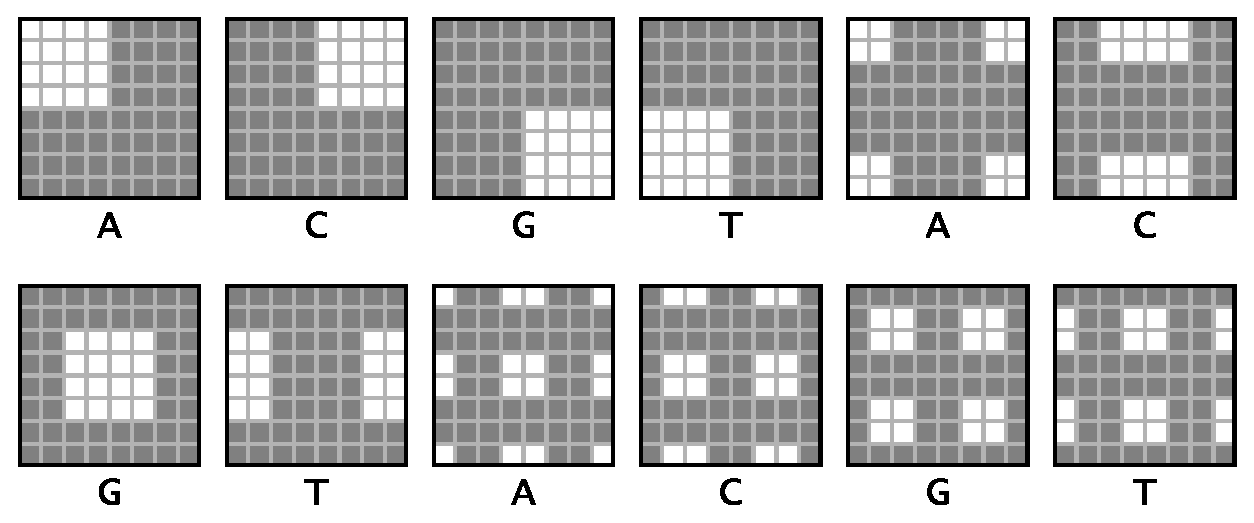
\includegraphics[width=\textwidth]{place/uniform_masks}}}
\end{picture}
\caption{\label{fig:uniform_masks}%
  Masks for the $8\times 8$ uniform array of Figure~\ref{fig:uniform_placement}
  when probes are synchronously embedded into \{ACGT\}$^{3}$. Masked spots are
  represented by shaded squares, unmasked spots by white squares. Note that
  masks of the same cycle have the same number of border conflicts.}
\end{figure}

%%%%%%%%%%%%%%%%%%%%%%%%%%%%%%%%%%%%%%%%%%%%%%%%%%%%%%%%%%%%%%%%%%%%%%%%%%%%%%%%
\section{TSP and threading algorithms}
\label{sec:placement_threading}

The border length problem on arrays of arbitrary probes was first discussed by
\citet{Hannenhalli2002}. The article reports that the first Affymetrix chips
were designed using a heuristic for the traveling salesman problem (TSP). The
idea is to build a weighted graph with nodes representing probes, and edges
containing the Hamming distances between their embeddings (see Equation
\ref{eq:hamming}). A TSP tour on this graph is heuristically constructed and
\emph{threaded} on the array in a row-by-row fashion
(Figure~\ref{fig:threading}a).

For uniform arrays, every solution of the TSP corresponds to a (one-dimensional)
Gray code since consecutive elements in the tour differ in only one position,
thus minimizing border conflicts between neighboring probes. For general arrays,
a TSP solution also reduces border conflicts as consecutive probes in the tour
are likely to be similar. Threading the (one-dimensional) tour on a
two-dimensional chip, row-by-row, on a leads to an arrangement where consecutive
probes in the same row have few border conflicts, but probes in the same column
may have very different embeddings.

Another problem of this approach is that the TSP is known to be NP-hard
\citep{Gross2004}, so computing an optimal TSP tour even for a small
$300\times 300$ array is not feasible, and only fast approximation algorithms
are suitable. In practice, Hannenhalli et.~al.\ managed to achieve
marginal improvements in tour cost using the 2-opt algorithm for TSP of
\citet{Lin1973} and an algorithm for weighted matching due to \citet{Gabow1976}.
Unfortunately, their efforts resulted in only $1.05\%$ reduction in tour cost
for a chip with $66\,000$ probes when compared to the greedy TSP algorithm
initially used at Affymetrix.

\begin{figure}[t]\centering
\begin{picture}(435,130)
\put(-2,0){ \makebox(145,15){a)}}
\put(147,0){\makebox(145,15){b)}}
\put(292,0){\makebox(145,15){c)}}
\put(-2,15){ \makebox(145,115){\includegraphics[width=0.3\textwidth]{0threading}}}
\put(147,15){\makebox(145,115){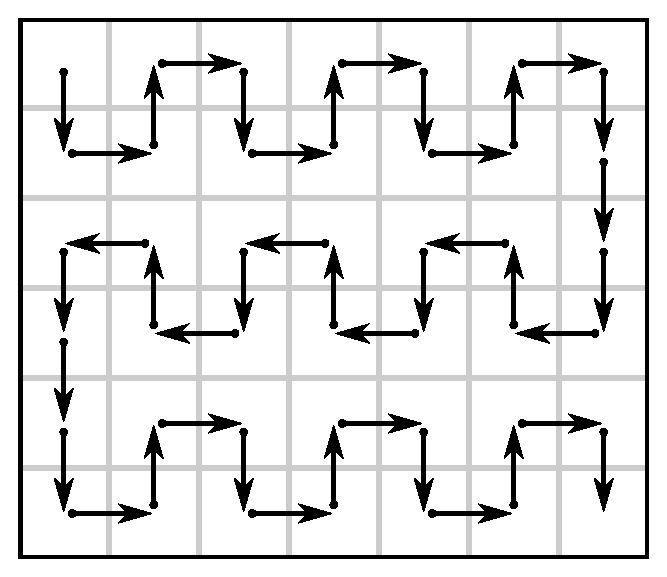
\includegraphics[width=0.3\textwidth]{1threading}}}
\put(292,15){\makebox(145,115){\includegraphics[width=0.3\textwidth]{2threading}}}
\end{picture}
\caption{\label{fig:threading}%
  Different ways of \emph{threading} probes on a chip. a) Standard row-by-row
  (0-threading); b) 1-threading; c) 2-threading.}
\end{figure}

Since improvements in the cost of the TSP tour seemed unlikely, Hannenhalli
et.~al.\ turned their attention to the problem of threading the tour on the
chip. They studied several threading alternatives, which they collectively
called \emph{$k$-threading} (Figure~\ref{fig:threading}). A $k$-threading is a
variation of the standard row-by-row threading, in which the right-to-left and
left-to-right paths are interspaced with alternating upward and downward
movements over $k$ sites (the row-by-row threading can be seen as a
$k$-threading with $k=0$); $k$ is called the \emph{amplitude} of the threading.
Hannenhalli et.~al.\ experimentally observed that 1-threading may reduce total
border length of layouts constructed with TSP tours in up to 20\% for large
chips when compared to row-by-row threading.

From now on, we will use the term TSP\,+$k$-threading to refer to the method of
computing a TSP tour and threading it on the array using $k$-threading.

%%%%%%%%%%%%%%%%%%%%%%%%%%%%%%%%%%%%%%%%%%%%%%%%%%%%%%%%%%%%%%%%%%%%%%%%%%%%%%%%
\section{Epitaxial placement}
\label{sec:placement_epitaxial}

A different strategy inspired by techniques used in the design of VLSI circuits,
called Epitaxial placement, or \emph{seeded crystal growth}, was proposed by
\citet{Kahng2002}. It essentially grows a placement around a single starting
``seed'' using a greedy heuristic. Although it was originally designed for chips
with synchronous embeddings, it can be trivially implemented for asynchronous
embeddings as well.

The algorithm starts by placing a random probe in the center of the array and
continues to insert probes in spots adjacent to already-filled spots. Priority
is given to spots whose all four neighbors are filled, in which case a probe
with the minimum number of border conflicts with the neighbors is placed.
Otherwise, all spots with $1 \leq i < 4$ filled neighbors are examined. For each
spot $s$, the algorithm finds a non-assigned probe~$p$ whose number of border
conflicts with the filled neighbors of $s$, $c(s,p)$, is minimal and assigns a
normalized cost $\bar{c}(s,p) := \sigma_i \cdot c(s,p) / i$ for this assignment,
where $0 < \sigma_i \leq 1$ are scaling coefficients (the authors propose
$\sigma_1 = 1$, $\sigma_2 = 0.8$, and $\sigma_3 = 0.6$). The assignment with
minimum $\bar{c}(s,p)$ is made and the procedure is repeated until all probes
have been placed.

In order to avoid repeated cost computations, the authors propose keeping a list
of probe candidates, for each spot, sorted by their normalized costs. This list
must be updated whenever one of its neighbors is filled; thus, it is updated at
most four times (but only two times on average).

With this algorithm, Kahng et.~al.\ claim a further 10\% reduction in
border conflicts over the TSP\,+\,1-threading approach of
\citet{Hannenhalli2002}. However, the Epitaxial algorithm has
at least quadratic time complexity as it examines every non-placed probe to fill
each spot, and large memory requirements if a list of probe candidates is kept
for each spot. Hence, like the TSP approach, it does not scale well to large
chips. In their experiments, the Epitaxial algorithm needed 274 seconds to
design a $100\times 100$ chip, but $4\,441$ seconds to design a $200\times 200$
chip. That is a $16.2$-fold increase in running time for a 4-fold increase in
number of spots. Chips of larger dimensions could not be computed because of
prohibitively large running time and memory requirements.

%%%%%%%%%%%%%%%%%%%%%%%%%%%%%%%%%%%%%%%%%%%%%%%%%%%%%%%%%%%%%%%%%%%%%%%%%%%%%%%%
\section{Sliding-Window Matching}
\label{sec:placement_swm}

\begin{figure}[t!]\centering
\centerline{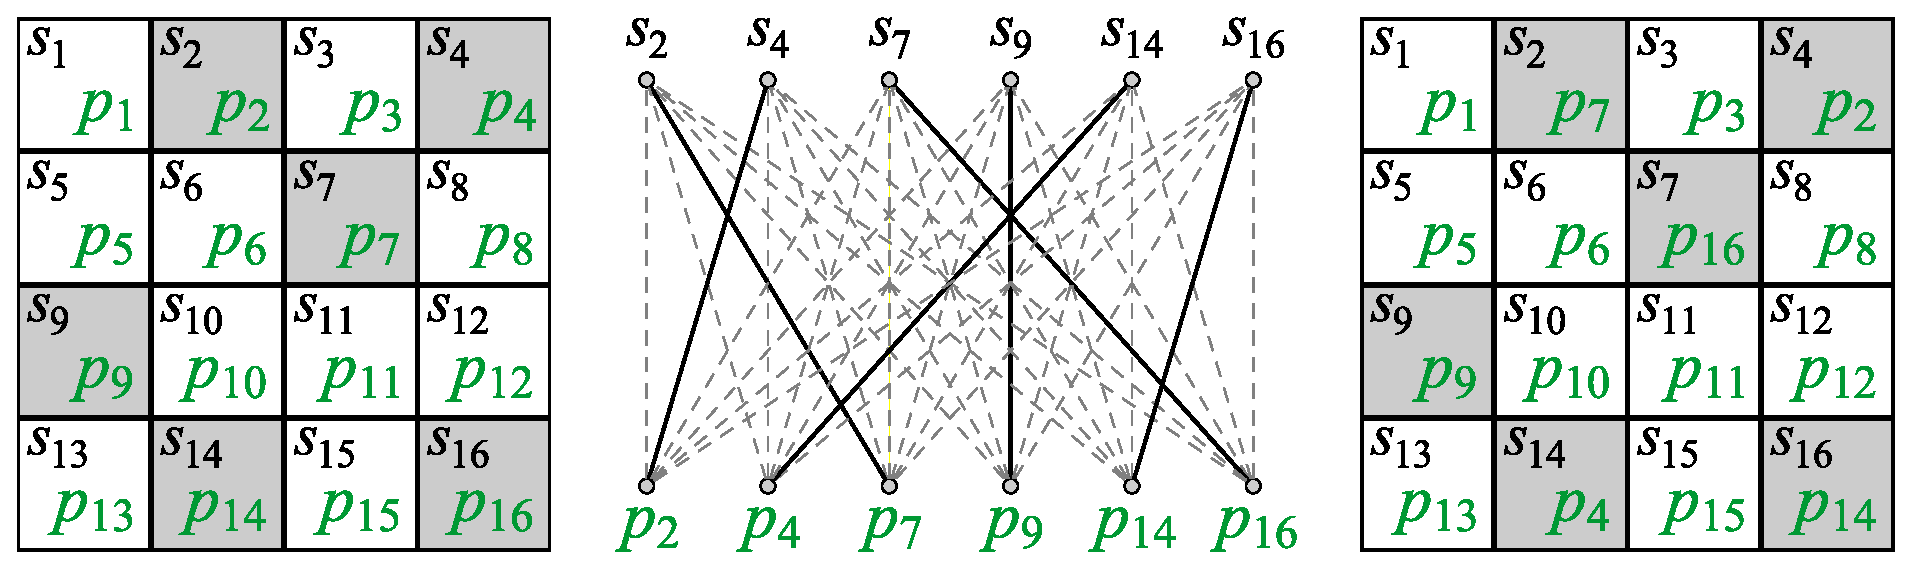
\includegraphics[width=\textwidth]{swm.eps}}
\begin{picture}(435,20)
\put(-3,0){ \makebox(125,20){a)}}
\put(139,0){\makebox(159,20){b)}}
\put(313,0){\makebox(125,20){c)}}
\end{picture}
\caption{\label{fig:swm}%
  Sliding-Window Matching algorithm. a) Initial arrangement of probes
  $p_1 \dots p_{16}$ inside a $4 \times 4$ window (with spots $s_1 \dots s_{16}$
  and a selected maximal independent set of spots (shaded). b) Bipartite graph
  with selected probes and spots, and a minimum weight perfect matching (dark
  edges) resulting in a minimum cost re-assignment of probes to spots. c) New
  arrangement inside the window according to the perfect matching.}%
\end{figure}

The Sliding-Window Matching algorithm \citep{Kahng2003}, SWM for short, is not
exactly a placement algorithm as it iteratively improves an existing placement
that can be constructed, for instance, by TSP\,+\,1-threading (Section
\ref{sec:placement_threading}).

The authors noted that the TSP tour can be conveniently substituted by
lexicographically sorting the probe sequences or, alternatively, their binary
embedding vectors with a linear-time radix sort. The sorting is faster, but it
is also likely to produce a worse initial placement than the TSP tour, with
consecutive embeddings being similar only in their first synthesis steps. The
authors argue that this is of little importance in practice given that this
placement is only used as a starting point for the SWM algorithm, and the
lexicographical sorting should be the choice for large microarrays because
computing a TSP tour takes prohibitively long for chips larger than
$500\times 500$ spots. (From now on, we will use the term
sorting\,+$k$-threading, or simply $k$-threading, to refer to the method of
sorting probes lexicographically and threading them on the array using
$k$-threading.)

As its name implies, SWM works inside a window that starts at the top left of
the chip and slides from left to right, top to bottom, while maintaining a
certain amount of overlap between each iteration. When the window reaches the
right-end of the chip, it is re-started at the left-end of the next set of rows,
also retaining an overlap with the preceding set of rows.

At each iteration, the algorithm attempts to reduce the total border length
inside the window by relocating some of its probes (Figure~\ref{fig:swm}a).
First, a random maximal independent set of spots is selected, and the probes
assigned to these spots are removed. The term independent refers to the fact
that selected spots can be re-assigned to probes without affecting the border
length of other selected spots. The algorithm then creates a bipartite graph
with nodes representing the removed probes and the now vacant spots
(Figure~\ref{fig:swm}b). The edges of this graph are weighted with the number of
border conflicts that are generated by the corresponding assignment.  Finally, a
minimum weight perfect matching on this graph is computed, and the indicated
assignments are made (Figure~\ref{fig:swm}c).

A minimum weight perfect matching requires polynomial time \citep{Gross2004},
but the small graphs generated by SWM can be computed rather quickly. The
authors experimentally observed that the best results are obtained with small
window sizes (e.g. $6\times 6$) and an overlap of half the window size.
Moreover, employing less effort in each window and executing more cycles of
optimization gives better results than more effort in each window and less
cycles.

Selecting an independent set of spots ensures that the cost of each new
assignment can be computed independently of the other assignments. The SWM was
designed for border length minimization (BLM) and it takes advantage of the fact
that, in this model, an independent set of spots can be constructed by selecting
spots that do not share a common border. SWM can be adapted for conflict index
minimization (CIM) by using larger windows containing relatively sparse
independent sets (to our knowledge, this has not been implemented yet).
Therefore several random independent sets should be constructed before moving
the window.

%%%%%%%%%%%%%%%%%%%%%%%%%%%%%%%%%%%%%%%%%%%%%%%%%%%%%%%%%%%%%%%%%%%%%%%%%%%%%%%%
\section{Row-Epitaxial}
\label{sec:placement_reptx}

Row-Epitaxial \citep{Kahng2003} is a variant of the Epitaxial algorithm with two
main differences introduced to improve scalability: i) spots are filled in a
pre-defined order, namely, from top to bottom, left to right, and ii) only a
limited number $Q$ of probe candidates are considered for filling each spot.

Like SWM, Row-Epitaxial improves an initial placement that can be constructed
by, for example, sorting\,+\,1-threading. For each spot $s$ with a probe $p$,
it looks at the next $Q$ probes that lie in close proximity (to the right or
below $s$), and swaps $p$ with the probe that generates the minimum number of
border conflicts between $s$ and its left and top neighbors.

In the experiments conducted by \citet{Kahng2003}, Row-Epitaxial was the best
large-scale placement algorithm (for BLM), achieving up to 9\% reduction in
border conflicts over TSP\,+\,1-threading, whereas SWM achieved slightly
worse results but required significantly less time.

Row-Epitaxial can also be adapted to CIM by swapping a probe of a spot $s$ with
the probe candidate that minimizes the sum of conflict indices in a region
around $s$ restricted to those neighboring probes that are to the left or above
$s$ (those which have already found their final positions).

Table~\ref{tab:reptx} shows the results of using Row-Epitaxial for both border
length and conflict index minimization on chips with random probe sequences
(uniformly generated). Probes were lexicographically sorted and left-most
embedded into the standard 74-step Affymetrix deposition sequence and threaded
on the array with $k$-threading. The resulting layouts were then used as a
starting point for Row-Epitaxial.

Although \citet{Hannenhalli2002} suggested 1-threading for laying out a TSP tour
on the chip, our results show that increasing the threading's amplitude from
$k=0$ to $k=4$ usually improves the initial layout produced by
sorting\,+\,$k$-threading, both in terms of border length and conflict index
minimization. For example, increasing the amplitude from $k=0$ to $k=4$ reduced
the normalized border length of the initial layout in up to $6.56\%$ (from
$23.6828$ to $22.1279$) and the average conflict index in up to $4.51\%$ (from
$689.6109$ to $658.5097$) on $800\times 800$ chips.

However, the best initial layouts rarely led to the best final layout produced
by Row-Epitaxial. With BLM the best results were usually achieved with $k=0$,
whereas with CIM there was no clear best value for $k$. In any case, the
difference due to varying $k$ for the threading were rather small for
Row-Epitaxial --- at most $0.78\%$ in normalized border length (from $16.9760$
with $k=0$ to $17.1085$ with $k=4$) and $0.26\%$ in average conflict index (from
$448.0140$ with $k=0$ to $449.1653$ with $k=4$), both on a $800\times 800$ chip
with $Q=5\,000$.

\begin{table}[p!]\centering
\caption{\label{tab:reptx}
  Normalized border length and average conflict index of layouts produced by
  Row-Epitaxial (Row-Eptx) on random chips of various dimensions, with initial
  layouts produced by sorting\,+\,$k$-threading. Running times are reported
  in minutes and include the time for $k$-threading and Row-Epitaxial. All
  results are averages over a set of five chips.}
\footnotesize{
\begin{tabular*}{\hsize}{crrlrrrlrrr}
\vspace{1pt}
     &     &     & & \multicolumn{3}{c}{Border length minimization} & & \multicolumn{3}{c}{Conflict index minimization} \\ \cline{5-7} \cline{9-11}
\vspace{1pt}
Dim. & $Q$ & $k$ & & $k$-threading & Row-Eptx & Time                & & $k$-threading & Row-Eptx & Time \\
\hline
$300\times 300$ &  5K & 0 &   &      24.9649  & {\bf 18.2935} &  1.1 &  &      701.8698  &      462.5194  &   4.9 \\
                &     & 1 &   &      24.1235  &      18.2999  &  1.3 &  &      690.8091  & {\bf 462.4656} &   5.1 \\
                &     & 2 &   &      23.8695  &      18.3072  &  1.2 &  &      685.5916  &      462.6394  &   4.6 \\
                &     & 3 &   &      23.7993  &      18.3226  &  1.2 &  &      683.5980  &      462.5885  &   5.1 \\
                &     & 4 &   & {\bf 23.7588} &      18.3279  &  1.3 &  & {\bf 682.3542} &      462.7775  &   5.1 \\
\cline{2-11}
                & 10K & 0 &   &      24.9649  & {\bf 18.1477} &  2.8 &  &      701.8698  &      444.0354  &   9.7 \\
                &     & 1 &   &      24.1235  &      18.1529  &  2.8 &  &      690.8091  &      444.0904  &   9.3 \\
                &     & 2 &   &      23.8695  &      18.1519  &  2.9 &  &      685.5916  &      444.1960  &  10.0 \\
                &     & 3 &   &      23.7993  &      18.1591  &  2.8 &  &      683.5980  & {\bf 443.9850} &  10.6 \\
                &     & 4 &   & {\bf 23.7588} &      18.1603  &  2.9 &  & {\bf 682.3542} &      444.1745  &   9.8 \\
\cline{2-11}
                & 20K & 0 &   &      24.9649  &      18.0274  &  7.2 &  &      701.8698  &      426.7824  &  18.9 \\
                &     & 1 &   &      24.1235  &      18.0325  &  6.9 &  &      690.8091  &      426.8863  &  18.5 \\
                &     & 2 &   &      23.8695  &      18.0277  &  6.6 &  &      685.5916  &      426.8832  &  19.3 \\
                &     & 3 &   &      23.7993  & {\bf 18.0272} &  6.6 &  &      683.5980  &      426.8694  &  19.6 \\
                &     & 4 &   & {\bf 23.7588} &      18.0321  &  7.5 &  & {\bf 682.3542} & {\bf 426.6600} &  20.2 \\
\hline
$500\times 500$ &  5K & 0 &   &      24.2693  & {\bf 17.6000} &  4.3 &  &      693.5428  &      456.2042  &  15.2 \\
                &     & 1 &   &      23.3454  &      17.6095  &  4.1 &  &      682.2097  & {\bf 456.1341} &  15.2 \\
                &     & 2 &   &      23.0797  &      17.6246  &  4.3 &  &      676.4884  &      456.5261  &  14.1 \\
                &     & 3 &   &      22.9632  &      17.6474  &  3.8 &  &      672.8160  &      456.5337  &  14.1 \\
                &     & 4 &   & {\bf 22.9162} &      17.6670  &  3.7 &  & {\bf 671.2636} &      456.8203  &  15.3 \\
\cline{2-11}
                & 10K & 0 &   &      24.2693  & {\bf 17.4503} & 13.1 &  &      693.5428  &      438.7075  &  33.9 \\
                &     & 1 &   &      23.3454  &      17.4523  & 12.8 &  &      682.2097  &      438.7379  &  33.6 \\
                &     & 2 &   &      23.0797  &      17.4582  & 12.7 &  &      676.4884  & {\bf 438.6477} &  30.4 \\
                &     & 3 &   &      22.9632  &      17.4685  & 12.5 &  &      672.8160  &      438.8183  &  30.8 \\
                &     & 4 &   & {\bf 22.9162} &      17.4755  & 12.5 &  & {\bf 671.2636} &      438.9280  &  32.8 \\
\cline{2-11}
                & 20K & 0 &   &      24.2693  &      17.3303  & 28.2 &  &      693.5428  &      421.1358  &  66.7 \\
                &     & 1 &   &      23.3454  & {\bf 17.3297} & 29.0 &  &      682.2097  &      421.1580  &  63.6 \\
                &     & 2 &   &      23.0797  &      17.3308  & 27.4 &  &      676.4884  &      421.1087  &  67.7 \\
                &     & 3 &   &      22.9632  &      17.3344  & 27.4 &  &      672.8160  & {\bf 420.9758} &  65.1 \\
                &     & 4 &   & {\bf 22.9162} &      17.3376  & 27.7 &  & {\bf 671.2636} &      421.0436  &  64.2 \\
\hline
$800\times 800$ &  5K & 0 &   &      23.6818  & {\bf 16.9760} & 12.2 &  &      689.6109  & {\bf 448.0140} &  36.9 \\
                &     & 1 &   &      22.6092  &      16.9927  & 12.2 &  &      672.2254  &      448.1474  &  40.3 \\
                &     & 2 &   &      22.3205  &      17.0187  & 11.7 &  &      664.9753  &      448.6130  &  38.6 \\
                &     & 3 &   &      22.1958  &      17.0589  & 11.7 &  &      660.5923  &      448.9159  &  40.2 \\
                &     & 4 &   & {\bf 22.1279} &      17.1085  & 12.0 &  & {\bf 658.5097} &      449.1653  &  40.0 \\
\cline{2-11}
                & 10K & 0 &   &      23.6818  & {\bf 16.8032} & 37.0 &  &      689.6109  & {\bf 432.2283} &  88.2 \\
                &     & 1 &   &      22.6092  &      16.8111  & 39.1 &  &      672.2254  &      432.5153  &  91.4 \\
                &     & 2 &   &      22.3205  &      16.8235  & 37.7 &  &      664.9753  &      432.5031  &  85.8 \\
                &     & 3 &   &      22.1958  &      16.8353  & 37.7 &  &      660.5923  &      432.6652  &  90.1 \\
                &     & 4 &   & {\bf 22.1279} &      16.8622  & 39.0 &  & {\bf 658.5097} &      432.6980  &  91.9 \\
\cline{2-11}
                & 20K & 0 &   &      23.6818  & {\bf 16.6771} & 83.1 &  &      689.6109  & {\bf 415.6470} & 174.2 \\
                &     & 1 &   &      22.6092  &      16.6803  & 83.2 &  &      672.2254  &      415.7402  & 181.1 \\
                &     & 2 &   &      22.3205  &      16.6851  & 83.4 &  &      664.9753  &      415.6622  & 179.7 \\
                &     & 3 &   &      22.1958  &      16.6915  & 86.5 &  &      660.5923  &      415.7609  & 172.3 \\
                &     & 4 &   & {\bf 22.1279} &      16.7007  & 80.3 &  & {\bf 658.5097} &      415.7951  & 190.9 \\
\hline
\end{tabular*}}
\end{table}

Our results also confirm that the running time of Row-Epitaxial is approximately
$O(Qn)$, i.e., linear in the chip size, where $Q$ is a user-defined parameter
that controls the number of probe candidades examined for each spot. In this
way, solution quality can be traded for running time: More candidates yield
better layouts but also demand more time.

%%%%%%%%%%%%%%%%%%%%%%%%%%%%%%%%%%%%%%%%%%%%%%%%%%%%%%%%%%%%%%%%%%%%%%%%%%%%%%%%
\section{Greedy}
\label{sec:placement_greedy}

As discussed in the previous section, the best results obtained with
Row-Epitaxial rarely came from the best initial layouts (produced by
$k$-threading). This is probably because Row-Epitaxial ignores the probe order
used by $k$-threading when it looks for probe candidates to fill a certain spot
(Row-Epitaxial always looks for candidates in the next $Q$ spots, row-by-row,
regardless of how probes were threaded on the array). Another possible
disadvantage of the $k$-threading\,+\,Row-Epitaxial approach is that each swap
made by Row-Epitaxial shuffles the probes in the not-changed spots, destroying
the lexicographical order used during the threading.

In this section, we present a new placement algorithm, Greedy, that combines the
Row-Epitaxial greedy heuristic and a $k$-threading filling strategy in a single
phase, using a linked list of probes to maintain the probe order during the
whole placement. Like Row-Epitaxial, Greedy fills the spots in a greedy fashion,
i.e., for each spot $s$, it examines $Q$ probe candidates and chooses the one
that can be placed at $s$ with minimum cost (Greedy can also be easily
implemented for border length as well as for conflict index minimization).

There are two main differences to Row-Epitaxial. First, instead of (re-)filling
spots row-by-row, spots are filled with $k$-threading (there is no need for an
initial layout). Perhaps more importantly, Greedy sorts the probes
lexicographically and keeps them in a doubly-linked list. This list is used to
maintain the lexicographical order during placement. Moreover, it is also used
to improve the chances of finding a candidate having fewer conflicts with the
last placed probe (which will be its neighbor on the chip): Once a probe $p$ is
selected to fill a certain spot, it is removed from the list and the next search
of candidates examines the probes around $p$'s former position in the list,
e.g., $Q/2$ probes to the left and to the right of $p$.

Table~\ref{tab:greedy} shows the results of using Greedy for both border length
and conflict index minimization on the same set of (random) chips that have been
previously used for the experiments with Row-Epitaxial
(Table~\ref{tab:reptx}). The best layouts were always achieved with $k=0$.
Interestingly, increasing the amplitude of the threading from $k=1$ to $k=4$
always improved the results in terms of border length. In terms of conflict
index, increasing $k$ from 1 to 3 worsened the results; in most cases,
increasing it from 3 to 4 improved the results.

In terms of BLM, Greedy and Row-Epitaxial produced similar results, with the
best layout of Greedy being sometimes marginally better and sometimes marginally
worse than the best layout of Row-Epitaxial. In terms of CIM, however, Greedy
was constantly and significantly better than Row-Epitaxial, achieving up to
$5.65\%$ reduction in average conflic index (from $415.6470$ to $392.1786$) on a
$800\times 800$ chip with $Q=20\,000$.

In our results, Greedy was between $13.9\%$ and $59.9\%$ slower than
Row-epitaxial in the BLM case ($19.7\%$ on average), and between $3.7\%$
and $18.1\%$ in the CIM case (only $5.6\%$ on average). The difference between
Row-epitaxial and Greedy drops in the CIM case because the extra time spent in
computing the cost of each candidate is higher than in the BLM case, which
reduces the impact of the time required to keep the doubly-linked list.

\begin{figure}\centering
%%
\begin{picture}(438,200)\footnotesize{
  \put(0,0){\makebox(215,200){
    \includegraphics{place/tradeoff/bl}
  }}
  \put(223,0){\makebox(215,200){
    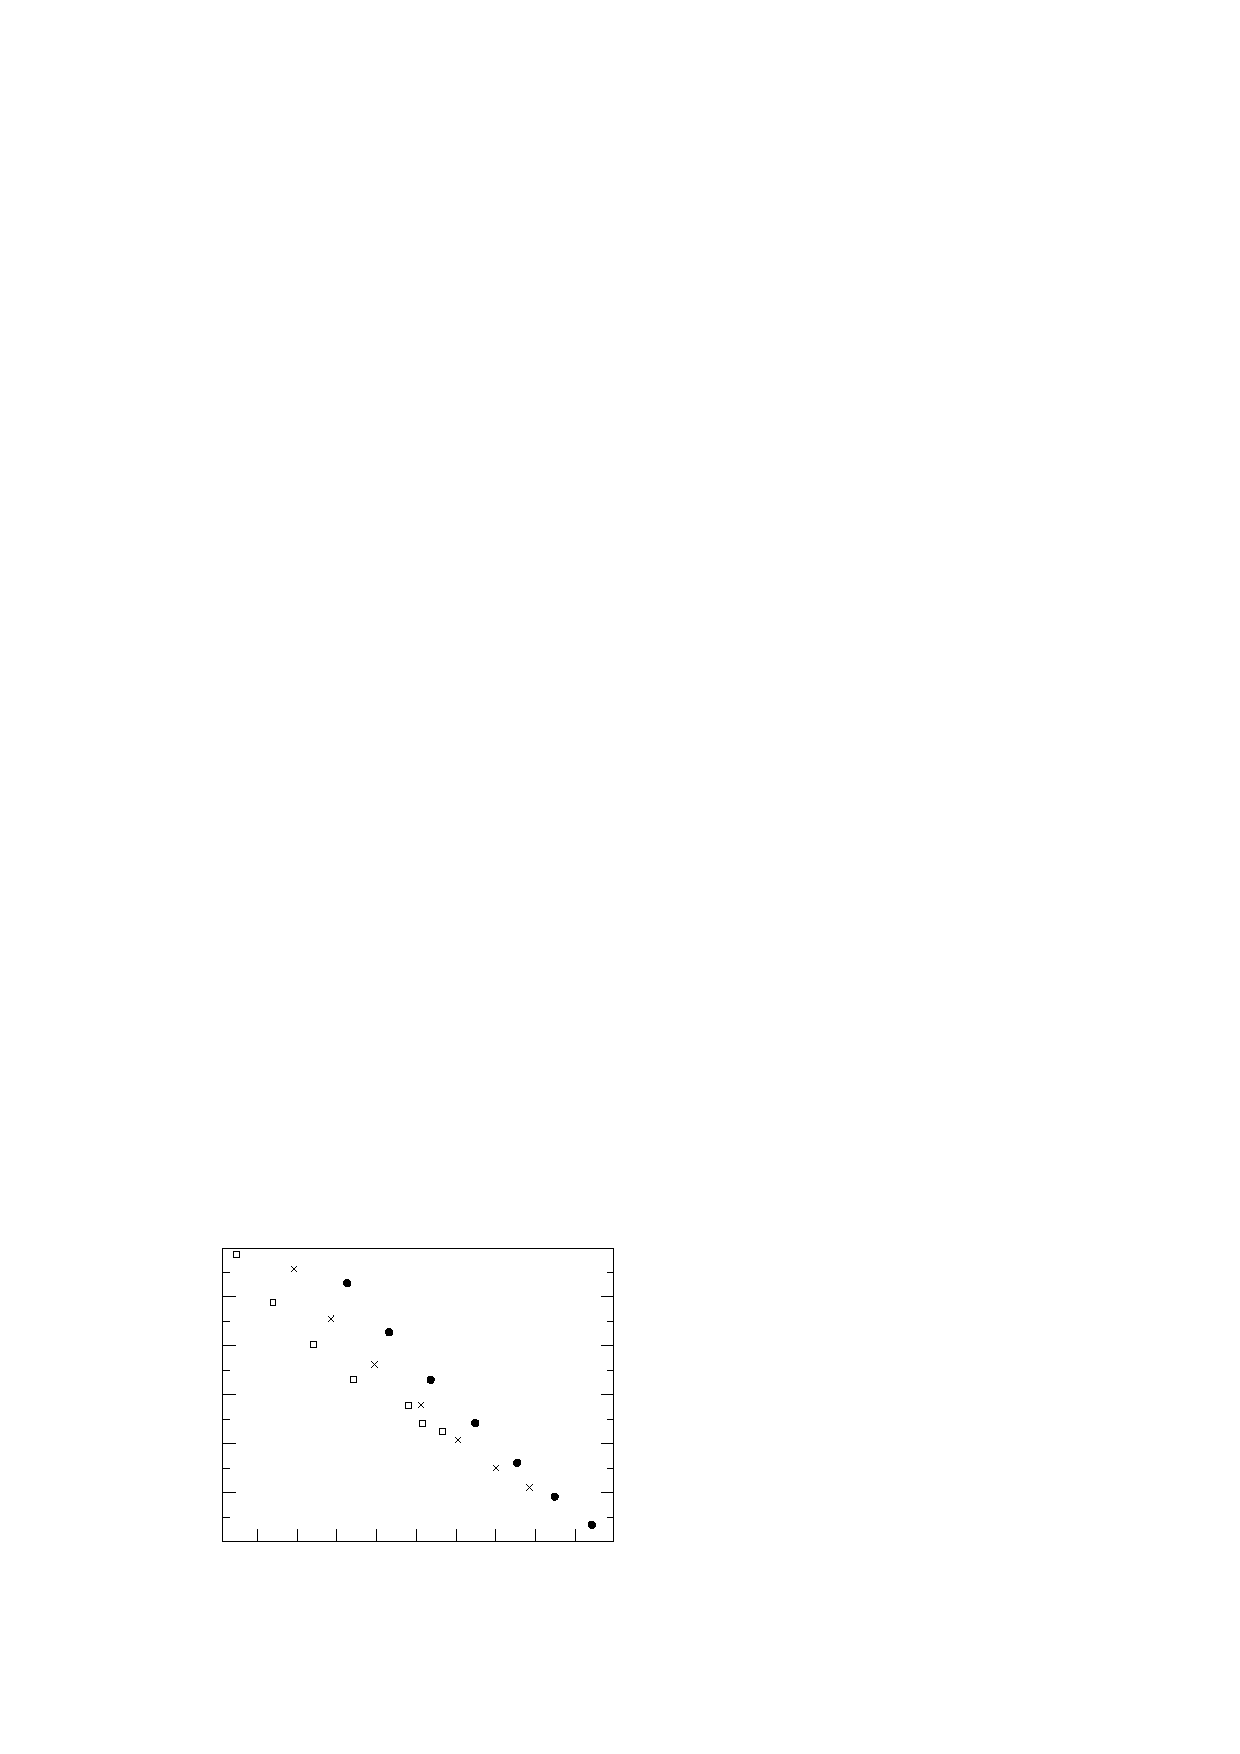
\includegraphics{place/tradeoff/ci}
  }}
}\end{picture}
%%
\caption{\label{fig:greedy_tradeoff}
  Trade-off between solution quality and running time (in logarithmic scale)
  with the Greedy algorithm on random chips of dimensions $300 \times 300$
  ({\tiny $\boxdot$}), $500 \times 500$ ({\tiny $\times$}) and $800 \times 800$
  ({\scriptsize $\bullet$}). The number $Q$ of candidates per spot are $1.25$K,
  $2.5$K, 5K, 10K, 20K, 40K, and 80K (from left to right). Layouts are measured
  by normalized border length (left) and average conflict index (right).}
\end{figure}

\begin{table}[p!]\centering
\caption{\label{tab:greedy}
  Normalized border length (NBL) and average conflict index (ACI) of layouts
  produced by Greedy on random chips of various dimensions. The results of
  Row-Epitaxial on the same set of chips (Table~\ref{tab:reptx}) is shown for
  comparison. Running times in minutes.}
\footnotesize{
\begin{tabular*}{\hsize}{crrrrrlrrrr}
\vspace{1pt}
     &         & \multicolumn{4}{c}{Border length minimization} & & \multicolumn{4}{c}{Conflict index minimization} \\ \cline{3-6} \cline{8-11}
\vspace{1pt}
     &         & \multicolumn{2}{c}{Row-Epitaxial} & \multicolumn{2}{c}{Greedy} & & \multicolumn{2}{c}{Row-Epitaxial} & \multicolumn{2}{c}{Greedy} \\
\vspace{1pt}
Dim. & $Q$ $k$ & NBL & Time & NBL & Time & & ACI & Time & ACI & Time \\
\hline
$300^2$ &  5K 0 & {\bf 18.2935} &  1.1 & {\bf 18.3182} &  1.6 &  &      462.5194  &   4.9 & {\bf 440.5166} &   5.4 \\
        &     1 &      18.2999  &  1.3 &      18.5037  &  1.6 &  & {\bf 462.4656} &   5.1 &      444.7837  &   5.3 \\
        &     2 &      18.3072  &  1.2 &      18.4222  &  1.6 &  &      462.6394  &   4.6 &      446.8662  &   5.3 \\
        &     3 &      18.3226  &  1.2 &      18.3863  &  1.6 &  &      462.5885  &   5.1 &      447.7464  &   5.0 \\
        &     4 &      18.3279  &  1.3 &      18.3728  &  1.5 &  &      462.7775  &   5.1 &      447.6559  &   5.3 \\
\cline{2-11}
        & 10K 0 & {\bf 18.1477} &  2.8 & {\bf 18.1830} &  4.3 &  &      444.0354  &   9.7 & {\bf 426.3480} &  10.9 \\
        &     1 &      18.1529  &  2.8 &      18.3912  &  4.7 &  &      444.0904  &   9.3 &      429.5617  &  11.3 \\
        &     2 &      18.1519  &  2.9 &      18.3058  &  4.5 &  &      444.1960  &  10.0 &      431.7555  &  11.1 \\
        &     3 &      18.1591  &  2.8 &      18.2732  &  4.6 &  & {\bf 443.9850} &  10.6 &      432.6821  &  11.3 \\
        &     4 &      18.1603  &  2.9 &      18.2415  &  4.6 &  &      444.1745  &   9.8 &      432.3800  &  11.0 \\
\cline{2-11}
        & 20K 0 &      18.0274  &  7.2 & {\bf 18.0576} &  9.6 &  &      426.7824  &  18.9 & {\bf 415.5003} &  30.3 \\
        &     1 &      18.0325  &  6.9 &      18.2813  &  9.2 &  &      426.8863  &  18.5 &      418.2357  &  21.3 \\
        &     2 &      18.0277  &  6.6 &      18.1985  &  9.2 &  &      426.8832  &  19.3 &      419.4866  &  21.1 \\
        &     3 & {\bf 18.0272} &  6.6 &      18.1617  &  9.5 &  &      426.8694  &  19.6 &      420.7345  &  20.1 \\
        &     4 &      18.0321  &  7.5 &      18.1328  &  8.8 &  & {\bf 426.6600} &  20.2 &      420.7332  &  21.0 \\
\hline
$500^2$ &  5K 0 & {\bf 17.6000} &  4.3 & {\bf 17.5830} &  5.8 &  &      456.2042  &  15.2 & {\bf 432.3023} &  15.9 \\
        &     1 &      17.6095  &  4.1 &      17.7842  &  5.3 &  & {\bf 456.1341} &  15.2 &      437.2417  &  16.2 \\
        &     2 &      17.6246  &  4.3 &      17.7087  &  5.3 &  &      456.5261  &  14.1 &      439.7432  &  15.6 \\
        &     3 &      17.6474  &  3.8 &      17.6759  &  5.4 &  &      456.5337  &  14.1 &      441.3441  &  16.2 \\
        &     4 &      17.6670  &  3.7 &      17.6561  &  5.4 &  &      456.8203  &  15.3 &      441.0668  &  16.1 \\
\cline{2-11}
        & 10K 0 & {\bf 17.4503} & 13.1 & {\bf 17.4673} & 15.8 &  &      438.7075  &  33.9 & {\bf 415.6951} &  35.4 \\
        &     1 &      17.4523  & 12.8 &      17.6765  & 16.0 &  &      438.7379  &  33.6 &      419.7788  &  33.4 \\
        &     2 &      17.4582  & 12.7 &      17.5936  & 16.8 &  & {\bf 438.6477} &  30.4 &      422.1943  &  36.3 \\
        &     3 &      17.4685  & 12.5 &      17.5550  & 16.2 &  &      438.8183  &  30.8 &      424.0554  &  34.6 \\
        &     4 &      17.4755  & 12.5 &      17.5324  & 15.7 &  &      438.9280  &  32.8 &      423.7936  &  35.2 \\
\cline{2-11}
        & 20K 0 &      17.3303  & 28.2 & {\bf 17.3554} & 33.3 &  &      421.1358  &  66.7 & {\bf 401.4609} &  67.1 \\
        &     1 & {\bf 17.3297} & 29.0 &      17.5829  & 34.0 &  &      421.1580  &  63.6 &      404.9949  &  69.8 \\
        &     2 &      17.3308  & 27.4 &      17.4939  & 34.1 &  &      421.1087  &  67.7 &      406.9576  &  67.8 \\
        &     3 &      17.3344  & 27.4 &      17.4519  & 34.7 &  & {\bf 420.9758} &  65.1 &      408.5048  &  69.4 \\
        &     4 &      17.3376  & 27.7 &      17.4273  & 33.7 &  &      421.0436  &  64.2 &      408.4556  &  68.4 \\
\hline
$800^2$ &  5K 0 & {\bf 16.9760} & 12.2 & {\bf 16.9124} & 15.3 &  & {\bf 448.0140} &  36.9 & {\bf 426.0757} &  41.9 \\
        &     1 &      16.9927  & 12.2 &      17.1259  & 15.5 &  &      448.1474  &  40.3 &      430.9759  &  42.7 \\
        &     2 &      17.0187  & 11.7 &      17.0551  & 15.1 &  &      448.6130  &  38.6 &      433.8504  &  42.9 \\
        &     3 &      17.0589  & 11.7 &      17.0214  & 15.4 &  &      448.9159  &  40.2 &      435.4797  &  43.3 \\
        &     4 &      17.1085  & 12.0 &      17.0009  & 15.4 &  &      449.1653  &  40.0 &      435.2589  &  43.2 \\
\cline{2-11}
        & 10K 0 & {\bf 16.8032} & 37.0 & {\bf 16.7951} & 45.5 &  & {\bf 432.2283} &  88.2 & {\bf 408.3982} &  91.4 \\
        &     1 &      16.8111  & 39.1 &      17.0122  & 43.2 &  &      432.5153  &  91.4 &      412.9971  &  95.1 \\
        &     2 &      16.8235  & 37.7 &      16.9333  & 45.1 &  &      432.5031  &  85.8 &      415.7934  &  91.7 \\
        &     3 &      16.8353  & 37.7 &      16.8935  & 45.9 &  &      432.6652  &  90.1 &      417.5229  &  95.2 \\
        &     4 &      16.8622  & 39.0 &      16.8748  & 45.6 &  &      432.6980  &  91.9 &      417.5098  &  91.3 \\
\cline{2-11}
        & 20K 0 & {\bf 16.6771} & 83.1 & {\bf 16.6980} & 95.8 &  & {\bf 415.6470} & 174.2 & {\bf 392.1786} & 186.4 \\
        &     1 &      16.6803  & 83.2 &      16.9263  & 93.2 &  &      415.7402  & 181.1 &      396.3923  & 185.9 \\
        &     2 &      16.6851  & 83.4 &      16.8376  & 93.8 &  &      415.6622  & 179.7 &      399.0043  & 186.9 \\
        &     3 &      16.6915  & 86.5 &      16.7947  & 94.4 &  &      415.7609  & 172.3 &      400.7189  & 183.3 \\
        &     4 &      16.7007  & 80.3 &      16.7727  & 97.2 &  &      415.7951  & 190.9 &      400.7257  & 189.3 \\
\hline
\end{tabular*}}
\end{table}

We also observed that, in terms of border length, increasing $Q$ above 5K has
little positive effect (see Figure~\ref{fig:greedy_tradeoff}). For instance, on
$800\times 800$ chips, increasing $Q$ from 5K to 20K reduced the normalized
border length by only $1.27\%$ (from $16.9124$ to $16.6980$ with $k=0$), while
requiring approximately six times more time. In terms of conflict index,
however, increasing $Q$ even above 40K still results in significant improvements
for large chips. For instance, on $800\times 800$ chips, increasing $Q$ from 40K
to 80K reduced the average conflict index by $3.18\%$ (from $378.3110$ to
$366.8446$ with $k=0$, data not shown).

The fact that increasing $Q$ has more effect in terms of conflict index is
probably because, in this measure, there is more room for optimization as the
conflicts can be moved to the extremities of the probes (while retaining the
same number of border conflicts) and a larger number of neighbors are involved.

Figure~\ref{fig:greedy_blm} shows the normalized border length per masking step
of layouts produced by Greedy for a $500\times 500$ chip with border length and
conflict index minimization. With BLM, the generated layout has most border
conflicts concentrated between steps 7 and 58. The last masks of this layout
have low levels of border conflicts because the probes are left-most embedded,
which leaves most embeddings in an unproductive state during the final synthesis
steps. As a result of the lexicographical sorting of probes, the first masks
also have relatively few conflicts. A representation of selected
photolithographic masks for this layout are shown in Figure
\ref{fig:greedy-bl_masks}. Layers of masked and unmasked regions that result
from sorting probes lexicographically can be seen in masks $M_1 \dots M_8$. Mask
$M_9 \dots M_{62}$ are very ``noisy'' as there seems to be little regularity in
their arrangement. From $M_{62}$ on, masks start to get ``darker'' as most
probes have been already fully synthesized.

With CIM, Greedy shifts border conflicts away from the steps that synthesize the
probes' middle bases (between steps 20 and 45; see Figure~\ref{fig:greedy_blm}),
which effectively reduces the average conflict index. Not surprinsingly, this
reduction comes at the expense of an increase in total border length --- the
normalized border length of this particular chip rose from $17.3513$ with BLM to
$19.8461$ with CIM. Figure~\ref{fig:greedy-ci_masks} shows a representation of
selected masks for this layout. Note that the first masks ($M_1 \dots M_4$)
still exhibit a ``layered'' structured, althought the layers are much narrower
and the masks noisier than the first masks of Figure~\ref{fig:greedy-bl_masks}.
In the middle masks $M_{20} \dots M_{45}$, especially between $M_{25}$ and
$M_{40}$, it is possible to see clusters of masked and unmasked spots that cause
the reduction in average conflict index.

\begin{figure}[t]\centering
\includegraphics{place/greedymasks/bl}
\caption{\label{fig:greedy_blm}%
  Normalized border length (on the left y-axis) per masking step
  of layouts produced by Greedy for a $500\times 500$ chip with border length
  ({\tiny $\times$}) and conflict index ({\tiny $\boxdot$}) minimization using
  $0$-threading and $Q=20$K. Chip contained random probe sequences left-most
  embedded in the standard 74-step Affymetrix deposition sequence. The number of
  middle bases synthesized at each step is shown in boxes (right y-axis).}
\end{figure}

\begin{figure}[p]\centering
%%
\begin{picture}(435,567)\footnotesize{
\put( -2,439){\makebox(145,128){
\includegraphics{place/greedymasks/bl/mask01}}}
\put(147,439){\makebox(145,128){
\includegraphics{place/greedymasks/bl/mask02}}}
\put(292,439){\makebox(145,128){
\includegraphics{place/greedymasks/bl/mask03}}}
\put( -2,429){\makebox(145, 10){$M_1$}}
\put(147,429){\makebox(145, 10){$M_2$}}
\put(292,429){\makebox(145, 10){$M_3$}}
\put( -2,296){\makebox(145,128){
\includegraphics{place/greedymasks/bl/mask04}}}
\put(147,296){\makebox(145,128){
\includegraphics{place/greedymasks/bl/mask05}}}
\put(292,296){\makebox(145,128){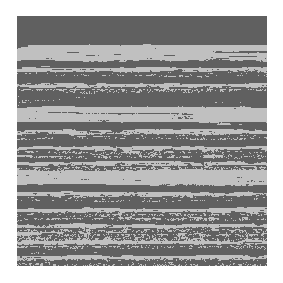
\includegraphics{place/greedymasks/bl/mask06}}}
\put( -2,286){\makebox(145, 10){$M_4$}}
\put(147,286){\makebox(145, 10){$M_5$}}
\put(292,286){\makebox(145, 10){$M_6$}}
\put( -2,153){\makebox(145,128){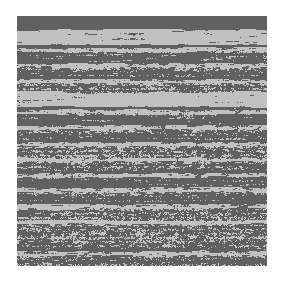
\includegraphics{place/greedymasks/bl/mask07}}}
\put(147,153){\makebox(145,128){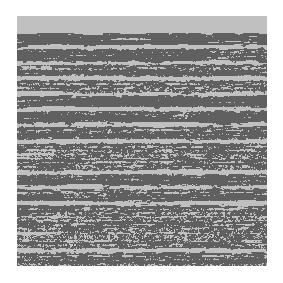
\includegraphics{place/greedymasks/bl/mask08}}}
\put(292,153){\makebox(145,128){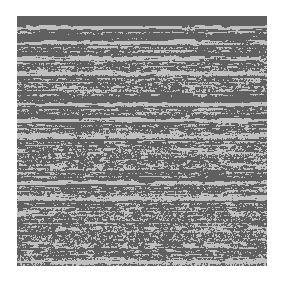
\includegraphics{place/greedymasks/bl/mask09}}}
\put( -2,143){\makebox(145, 10){$M_7$}}
\put(147,143){\makebox(145, 10){$M_8$}}
\put(292,143){\makebox(145, 10){$M_9$}}
\put( -2, 10){\makebox(145,128){
\includegraphics{place/greedymasks/bl/mask62}}}
\put(147, 10){\makebox(145,128){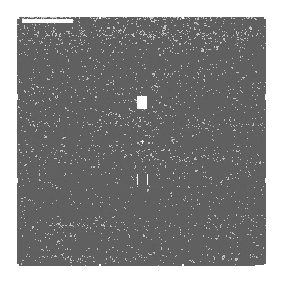
\includegraphics{place/greedymasks/bl/mask70}}}
\put(292, 10){\makebox(145,128){
\includegraphics{place/greedymasks/bl/mask74}}}
\put( -2,  0){\makebox(145, 10){$M_{62}$}}
\put(147,  0){\makebox(145, 10){$M_{70}$}}
\put(292,  0){\makebox(145, 10){$M_{74}$}}
}\end{picture}
%%
\caption{\label{fig:greedy-bl_masks}%
  Selected masks generated by Greedy with border length minimization for a
  random $500\times 500$ chip with 25-mer probes leftmost embedded in the
  standard Affymetrix deposition sequence. Unmasked (masked) spots are
  represented by light (dark) dots.}
\end{figure}

\begin{figure}[p]\centering
%%
\begin{picture}(435,567)\footnotesize{
\put( -2,439){\makebox(145,128){
\includegraphics{place/greedymasks/ci/mask01}}}
\put(147,439){\makebox(145,128){
\includegraphics{place/greedymasks/ci/mask02}}}
\put(292,439){\makebox(145,128){
\includegraphics{place/greedymasks/ci/mask03}}}
\put( -2,429){\makebox(145, 10){$M_1$}}
\put(147,429){\makebox(145, 10){$M_2$}}
\put(292,429){\makebox(145, 10){$M_3$}}
\put( -2,296){\makebox(145,128){
\includegraphics{place/greedymasks/ci/mask04}}}
\put(147,296){\makebox(145,128){
\includegraphics{place/greedymasks/ci/mask20}}}
\put(292,296){\makebox(145,128){
\includegraphics{place/greedymasks/ci/mask25}}}
\put( -2,286){\makebox(145, 10){$M_4$}}
\put(147,286){\makebox(145, 10){$M_{20}$}}
\put(292,286){\makebox(145, 10){$M_{25}$}}
\put( -2,153){\makebox(145,128){
\includegraphics{place/greedymasks/ci/mask30}}}
\put(147,153){\makebox(145,128){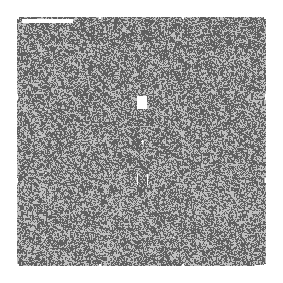
\includegraphics{place/greedymasks/ci/mask32}}}
\put(292,153){\makebox(145,128){
\includegraphics{place/greedymasks/ci/mask37}}}
\put( -2,143){\makebox(145, 10){$M_{30}$}}
\put(147,143){\makebox(145, 10){$M_{32}$}}
\put(292,143){\makebox(145, 10){$M_{37}$}}
\put( -2, 10){\makebox(145,128){
\includegraphics{place/greedymasks/ci/mask40}}}
\put(147, 10){\makebox(145,128){
\includegraphics{place/greedymasks/ci/mask45}}}
\put(292, 10){\makebox(145,128){
\includegraphics{place/greedymasks/ci/mask65}}}
\put( -2,  0){\makebox(145, 10){$M_{40}$}}
\put(147,  0){\makebox(145, 10){$M_{45}$}}
\put(292,  0){\makebox(145, 10){$M_{65}$}}
}\end{picture}
%%
\caption{\label{fig:greedy-ci_masks}%
  Selected masks generated by Greedy with conflict index minimization for a
  random $500\times 500$ chip with 25-mer probes leftmost embedded in the
  standard Affymetrix deposition sequence. Unmasked (masked) spots are
  represented by light (dark) dots.}
\end{figure}

%%%%%%%%%%%%%%%%%%%%%%%%%%%%%%%%%%%%%%%%%%%%%%%%%%%%%%%%%%%%%%%%%%%%%%%%%%%%%%%%
\section{Summary}
\label{sec:placement_summary}

In this chapter, we have surveyed placement algorithms for the Microarray Layout
Problem, including an optimal placement strategy for uniform arrays based on a
two-dimensional Gray code. For general arrays, we have presented more
experimental results with Row-Epitaxial, the best known placement algorithm to
date, and studied the impact of the choice of threading for its initial layout.

We have also introduced a new placement algorithm, Greedy. Greedy achieved
similar results in terms of BLM and better results in terms of CIM compared to
Row-Epitaxial. For BLM, Row-Epitaxial is faster than Greedy and should still be
the method of choice. For CIM, however, we believe that the improvements
achieved by Greedy over Row-Epitaxial justify the small increase in running
times.
